\chapter{Results and Discussion}

\section{Results}
The project had various critical phases that were completed. This section will present all the results generated relating to the major concepts of the project. This includes results relating to: system design, image processing, captured and processed data, modelling, and the EKF. All results are generated from an 18 second run completed with the designed system. This run generated 1800 data points, including a transient period from samples 0 to 200. Samples 400 to 1800 demonstrates steady state running.

\subsection{System Design Results}
The data capture system was designed to meet the specifications outlined in the methodology chapter. The device was comfortable, light weight and adjustable such that it could easily be used by a large variety of people. The device was also sturdy and well constructed allowing for long term usage. Pictured below is a subject wearing the data capture system.

\begin{figure}[!ht] 
\captionsetup{width=0.8\linewidth, font=small}  
\includegraphics[width=1\linewidth]{figures/pat_harness.png}
\caption{subject wearing the motion capture system }
\label{fig:pat_harness}
\end{figure}

The stereo housings were fully functional and offered a good fit for both the cameras and the mounting hardware. Although the cameras moved during running they captured all the critical points in every single frame. The device in no way affected the gait of the subject as the system had a minimal footprint.

\subsection{Image Processing Results}
The video streams were successfully processed to extract all the critical data points from each frame. By using the DigitizingTools MATLAB package created by Hedrick et al. \cite{hedrick2008software} it was possible to accurately quantify the marker positions on the different video frames. 

\begin{figure}[!ht] 
\captionsetup{width=0.8\linewidth, font=small}  
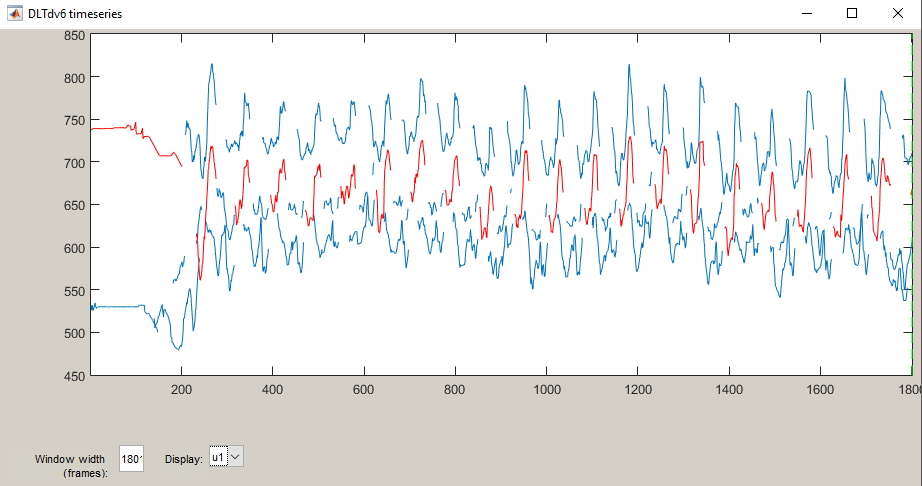
\includegraphics[width=0.8\linewidth]{figures/ipdatapattern.png}
\caption{iamge processing things}
\label{fig:ipdatapattern}
\end{figure}

The figure above shows the quantization of various points identified in the image frames of a single video stream. The frame number is displayed on the x-axis while the y-axis shows tracks the change in position of the $ (x,y) $ pixel values.

Four points were tracked in each video stream. since there were 4 cameras each tracking 4 points a total of 16 datasets were successfully created. 


\newpage
\subsection{Captured and Processed Data}
The following figure shows the pre EKF accelerometer data in the body frame. The x-axis represents the sample and the y-axis linear acceleration in $ m/s^2 $.

\begin{figure}[!ht] 
\captionsetup{width=0.8\linewidth, font=small}  
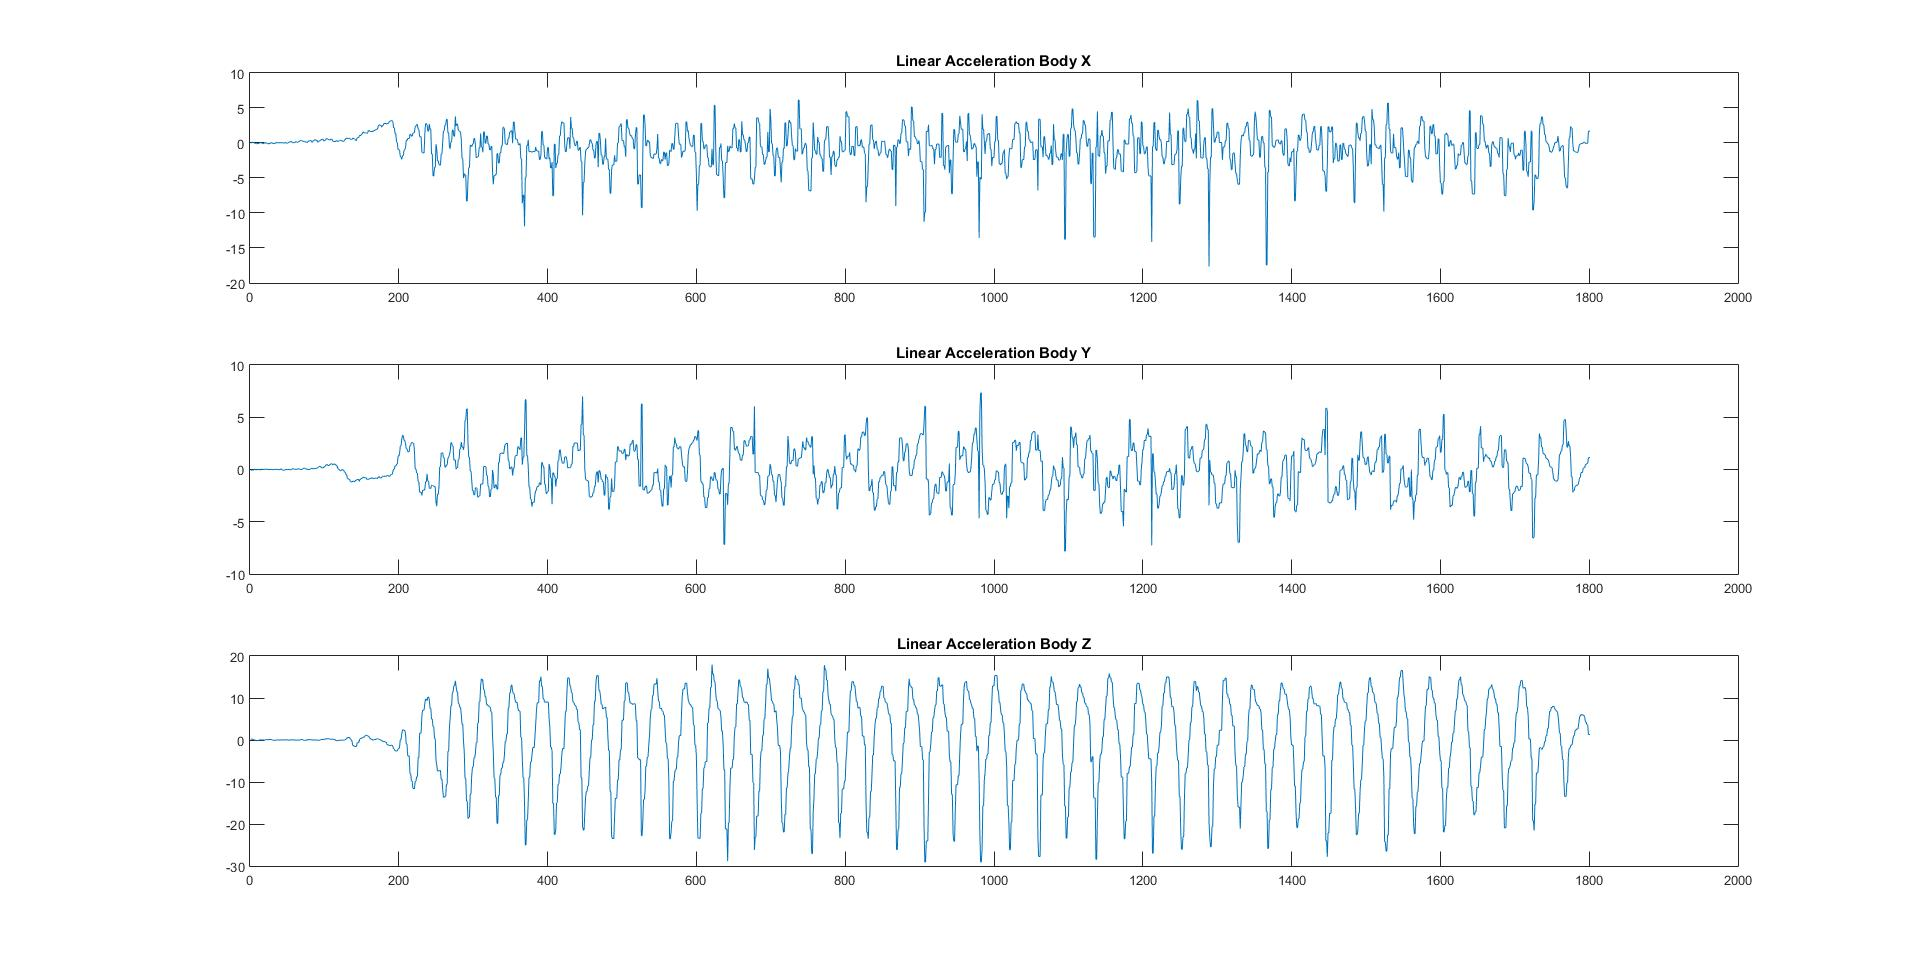
\includegraphics[width=1\linewidth]{figures/accelerometer.jpg}
\caption{Pre filter accelerometer data}
\label{fig:accelerometer}
\end{figure}

This figure shows the linear acceleration of the runner's body. The accelerometer data has been pre processed to remove the sensor bias. When looking at the Z axis accelerometer data we can clearly see a periodic motion correlating with the gait period of the subject. Some clear points of local minimum indicate when the runner made contact with the ground. These values were in the expected range of 3 to4 times the gravitational acceleration 

easily within the bounds of the sensors

The system was fully capable of capturing all the data necessary to quantify the gait of a runner. The following is a graph of the accelerometer in the z-body frame against time. From this graph it it the rhythmic motion of running is easy to see. a spike of close to 4g seen at the moment of impact and a maximum acceleration of around 1 g as the subject reaches maximum height.


\newpage
The following figure shows the pre EKF gyroscope data in the body frame. The x-axis represents the sample and the y-axis angular velocity in $ rad/s $.

\begin{figure}[!ht] 
\captionsetup{width=0.8\linewidth, font=small}  
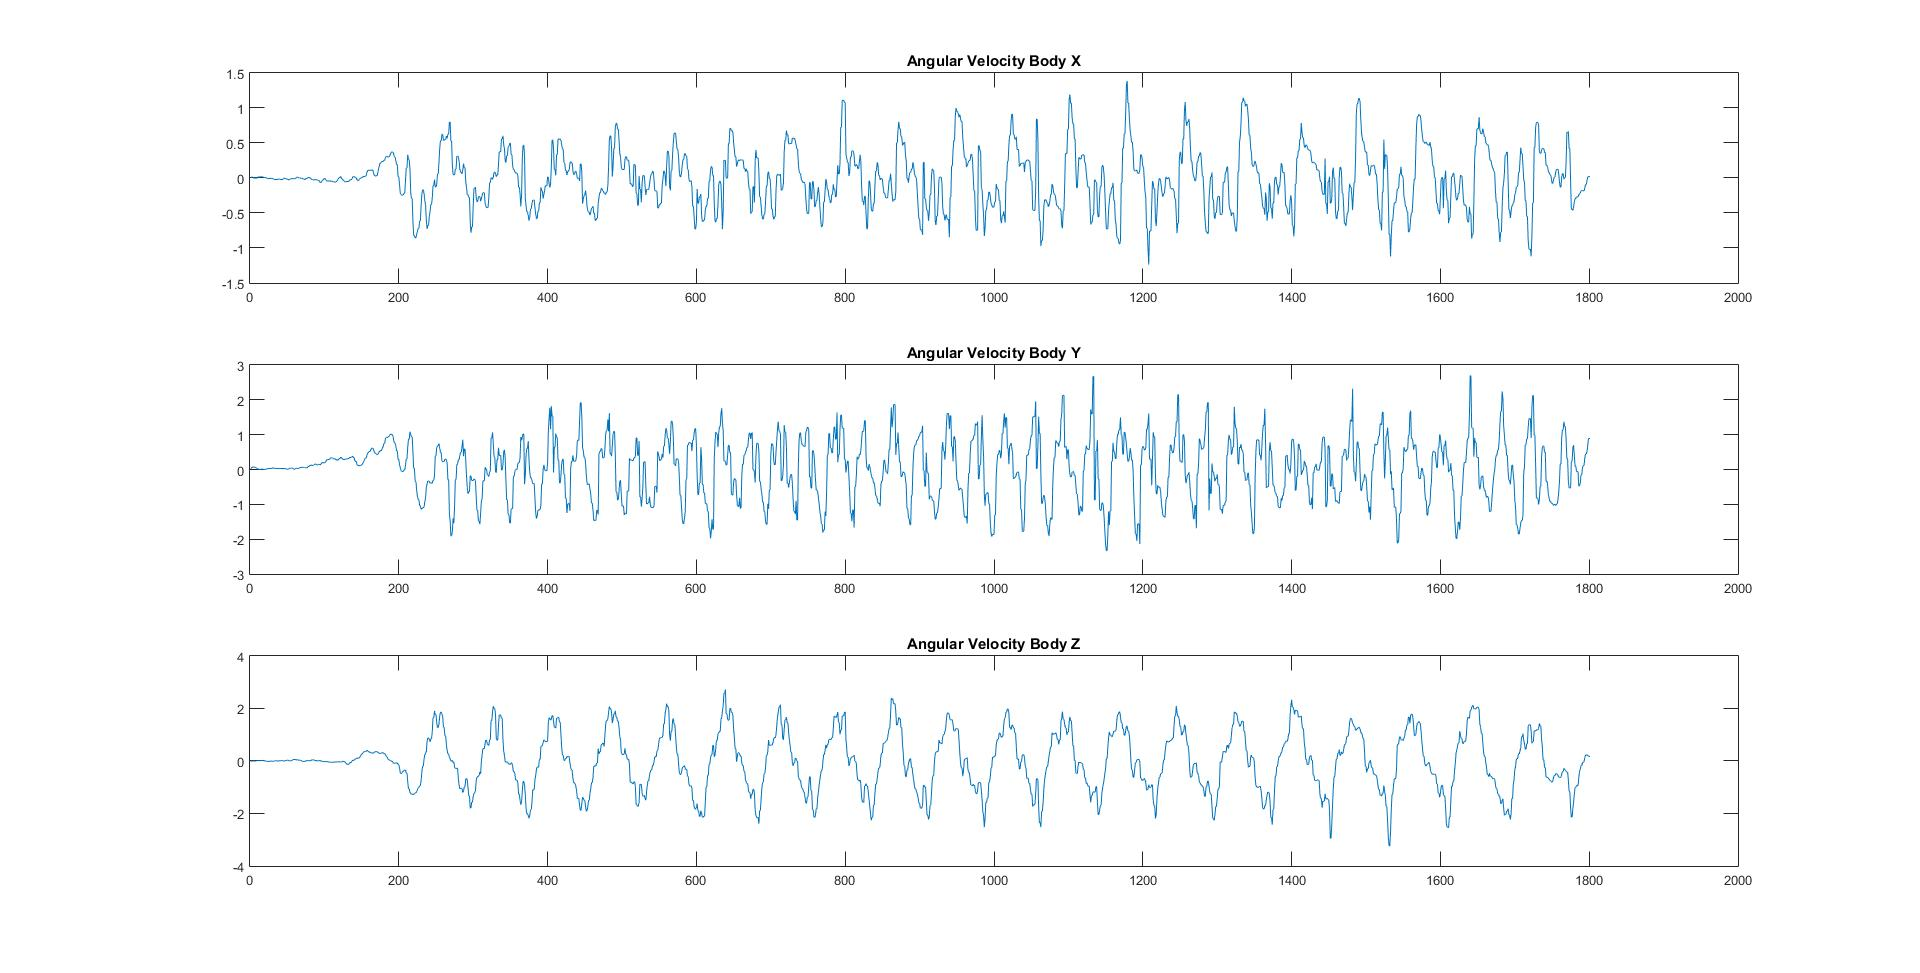
\includegraphics[width=1\linewidth]{figures/gyroscope.jpg}
\caption{Pre filter gyroscope data}
\label{fig:gyroscope}
\end{figure}

data bias removed


\newpage
The following figure shows the pre EKF magnetometer data in the body frame. The x-axis represents the sample and the y-axis magnetic flux density in $ microTesla $.

\begin{figure}[!ht] 
\captionsetup{width=0.8\linewidth, font=small}  
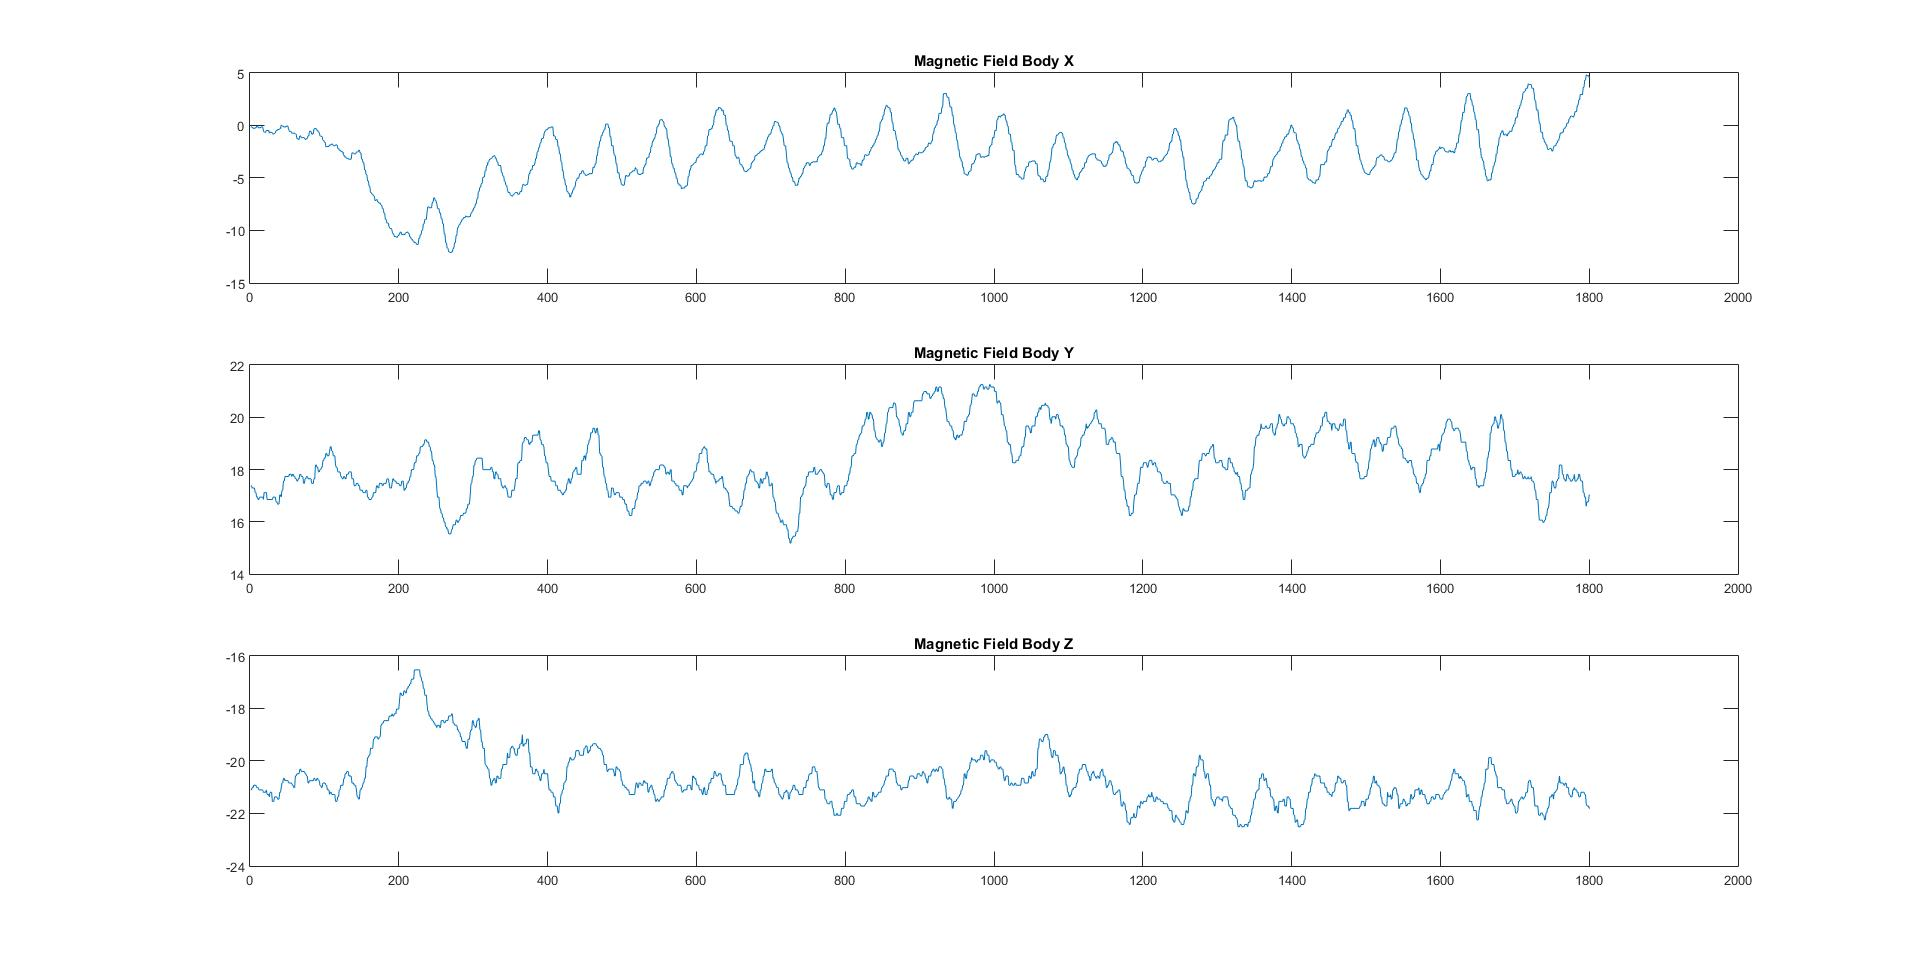
\includegraphics[width=1\linewidth]{figures/magnetometer.jpg}
\caption{Pre filter magnetometer data}
\label{fig:magnetometer}
\end{figure}

cannot have bias removed.

\newpage

The x-axis of the GPS Position graph represents position in the x direction and the y-axis the position in the y direction of the body with respect to the inertial frame.

The x-axis of the GPS Velocity graph 

represents velocity in the x direction as blue and  

the velocity in the y direction in red 

of the body with respect to the inertial frame.

The barometer  plots the sample on the 



\begin{figure}[!ht] 
\captionsetup{width=0.8\linewidth, font=small}  
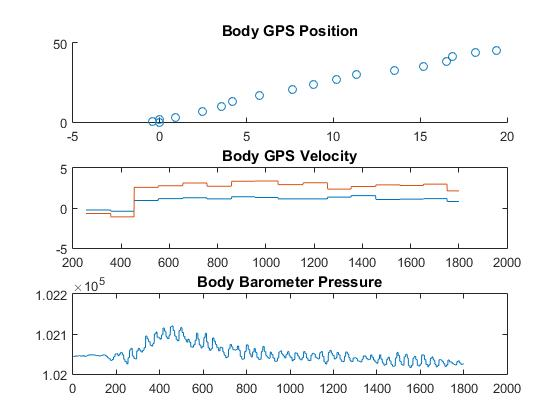
\includegraphics[width=1\linewidth]{figures/gps.jpg}
\caption{Pre filter GPS and barometer data}
\label{fig:gps}
\end{figure}

The GPS data shows the initial position (0,0) and the final position around (20,50)



\newpage


\begin{figure}[!ht] 
\captionsetup{width=0.8\linewidth, font=small}  
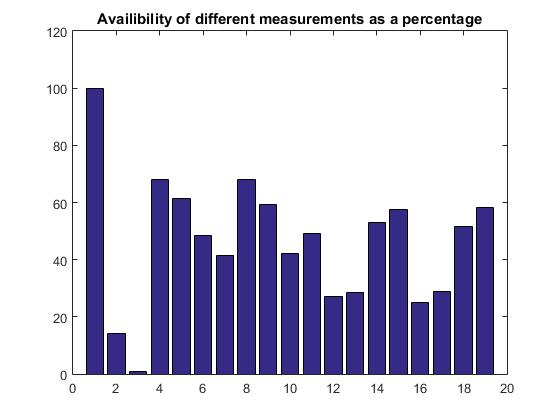
\includegraphics[width=0.75\linewidth]{figures/hist.jpg}
\caption{iamge processing things}
\label{fig:hist}
\end{figure}

\newpage
concluding remarks


\subsection{Model Results}



\subsection{EFK Results}



\section{Discussion}


\subsection{System Design}





\subsection{Image Processing}
The techniques of image processing considered in this thesis shows the difficulty in implementing an automated image processing system.


\subsection{Captured Data}


\subsection{System Modelling}
model was usable and back up by literature review.

The system model had 2 major shortcomings. Firstly the assumption of a rigid chest and secondly the assumption that the cameras stay aligned with the body frame.

It is clear from the Gyroscope data that the chest of a runner oscillates. Since the cameras protrude from the chest they move in an arc pattern in space. 

The model proved sufficient

talk about how the model would also allow the sensor to be used for subjects with prosthesis and allow for better understanding of disabled persons.


\subsection{Extended Kalman Filter}
The filter had limited results
\cite{gps}











